\documentclass[10pt,a4paper]{article}
\usepackage[utf8]{inputenc}
\usepackage[italian]{babel}
\usepackage{amsmath}
\usepackage{amsfonts}
\usepackage{amssymb}
\usepackage{graphicx}
\usepackage[left=2cm,right=2cm,top=2cm,bottom=2cm]{geometry}
\newcommand{\rem}[1]{[\emph{#1}]}

\author{Gruppo AC \\ Federico Belliardo, Giulia Franchi, Francesco Mazzoncini}
\title{Esercitazione N.7: Usi non lineari dell’ OpAmp}
\begin{document}

\maketitle
Questa esperienza ha come obbiettivo quello di studiare il funzionamento di un amplificatore operazionale modello TL081 in circuiti non lineari.

\section*{A. Discriminatore}

Si è montato il circuito in fig. \ref{circuito1}, utilizzando $V_{CC} = 14.96\pm0.08 \, V$ e $V_{EE} = 14.96 \pm 0.08 \, V$ come tensioni di alimentazione.

\begin{figure}[h]
\centering
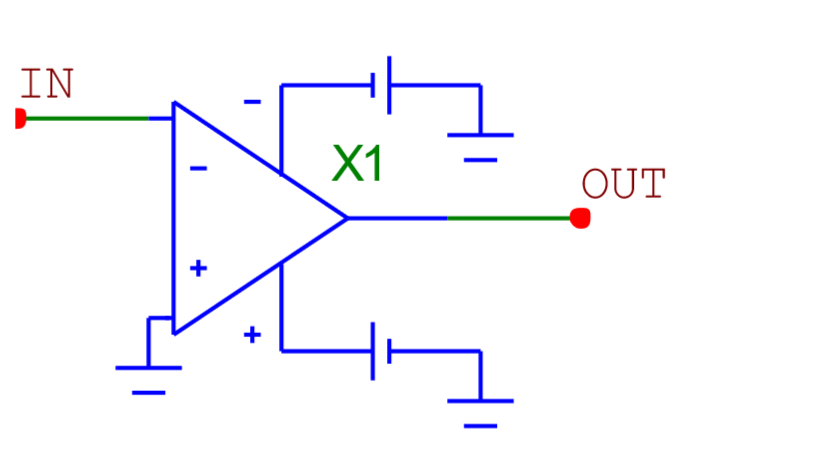
\includegraphics[scale=0.5]{Discriminatore.png}
\caption{Discriminatore realizzato con un OpAmp modello TL081.}
\label{circuito1}
\end{figure}

Si è studiata la risposta del circuito ad un segnale sinusoidale. Il circuito ideale dovrebbe funzionare come un comparatore che rileva se la tensione è positiva o negativa, infatti il segnale in ingresso viene invertito e amplificato in modo da mandare in saturazione l'uscita alla tensione di alimentazione  positiva o negativa a seconda del segno dell'ingresso.\\
Per basse frequenze il comportamento è quello ideale del discriminatore (l'uscita è un'onda quadra), come si vede in fig.\ref{funzionaBene}.

\begin{figure}[h]
\centering
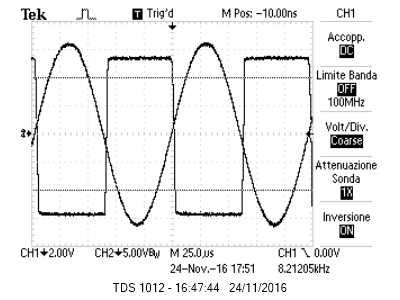
\includegraphics[scale=1.0]{immagini/discriminatore.png}
\caption{Segnale in ingresso e in uscita (invertito) del circuito discriminatore.}
\label{funzionaBene}
\end{figure}

Purtroppo il circuito da noi analizzato non è un amplificatore ideale e come tale presenta dei limiti al suo funzionamento.\\
Come primo limite vediamo l'influenza della tensione di offset $V_{OS}$, che dalla fig. \ref{Vos} è stimata essere $V_{OS} = 25.6 \pm 0.8 \, mV$.\\

\begin{figure}[h]
\centering
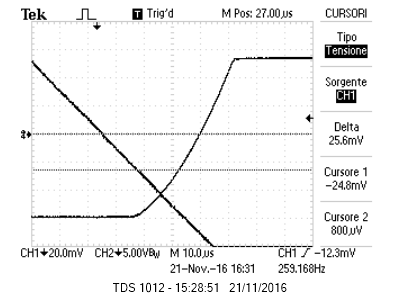
\includegraphics[scale=1.0]{immagini/Vos.png}
\caption{Misura della tensione di offset $V_{os}$}
\label{Vos}
\end{figure}

Inoltre all'aumentare della frequenza si notano gli effetti dello \emph{slew rate} finito dell'OpAmp. La pendenza delle rette che costituiscono la transizione tra uscita alta e bassa satura e il segnale diventa sempre più simile a un onda trapezoidale, per diventare poi un'onda triangolare, vedi fig. \ref{slewRate}.\\

\begin{figure}[h]
\centering
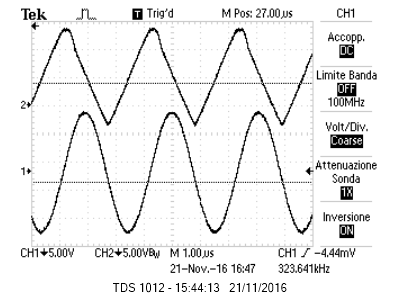
\includegraphics[scale=1.0]{immagini/slewRate.png}
\caption{Effetto dello \emph{slew rate} sull'uscita del discriminatore.}
\label{slewRate}
\end{figure}

Abbiamo valutato lo \emph{slew rate} con due misure di tensione e di tempo: $dV = 4.00 \pm 0.04 \, V$ e $dt = 336 \pm 4 \, ns$, da questa si ricava \emph{slew rate} = $11.9 \pm 0.4 \, \frac{V}{\mu s}$, questo valore è simile a quello trovato nell'esperienza precedente \emph{slew rate} = $11.4 \pm 0.6 \, \frac{V}{\mu s}$.\\

Ad alta frequenza e a basso segnale l'uscita ricorda il fenomeno di clipping inferiore (o superiore), come si vede in fig. \ref{clipping}.\\
Il valore a cui satura l'uscita dipende dal segno dell'offset (in continua) che il generatore di funzioni fornisce, infatti nell'opAmp un segnale a frequenza nulla viene integrato e l'uscita si satura alla tensione di alimentazione che ha segnale opposto all'offset.\\
Tuttavia con un'ampiezza ridotta il segnale può diminuire tanto da non mandare in saturazione l'uscita e allora si osserva che per un certo intervallo di tempo il segnale in uscita è sinusoidale (fig. \ref{clipping}).\\

\begin{figure}[h]
\centering
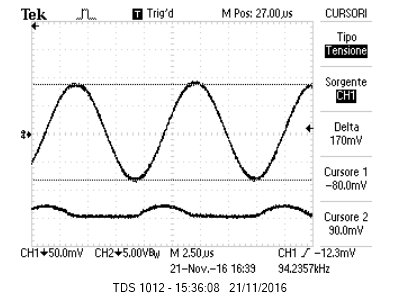
\includegraphics[scale=1.0]{immagini/prodottoBandaGuadagno2.png}
\caption{Segnale sinusoidale in ingresso ad alta frequenza.}
\label{clipping}
\end{figure}

E' addirittura possibile scegliere un segnale tanto piccolo in ampiezza da non mandare mai l'opAmp in saturazione, come si vede nelle fig. \ref{senoAlto} e fig. \ref{senoBasso}, riferiti a un caso di offset rispettivamente positivo e negativo.

Il comportamento descritto è consistente col fatto che alte frequenze il circuito si comporta da integratore (dove le impedenze sono da ricercarsi nelle giunzioni all'interno del'opAmp), dunque il segnale in uscita è sempre sinusoidale e sfasato. L'ampiezza diminuisce all'aumentare della frequenza come ci si aspetta per un circuito integratore. 

\begin{figure}[h]
\centering
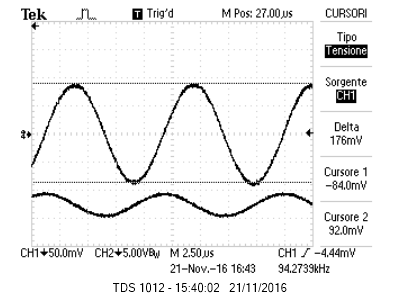
\includegraphics[scale=1.0]{immagini/sinusoidaleinBasso.png}
\caption{Segnale sinusoidale integrato con offset (in uscita) in basso.}
\label{senoBasso}
\end{figure}


\begin{figure}[h]
\centering
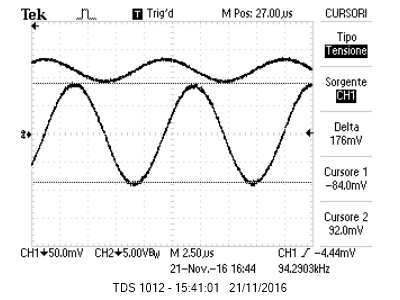
\includegraphics[scale=1.0]{immagini/sinusoidaleinAlto.png}
\caption{Segnale sinusoidale intgrarato con offset (in uscita) in alto.}
\label{senoAlto}
\end{figure}

In altri termini il comportamento da integratore si può spiegare invocando la finitezza del fattore GBW, che intruduce una frequenza di taglio nel sistema e una massima amplificazione alle basse frequenze. Il segnale in uscita è comunque limitato dalla tensioni $V_{CC}$ e $V_{EE}$ quindi non si può valutare con una misura l'ampificazione massima e pertanto risulta difficile dare un stima del prodotto $GBW = A_{max} * f_{taglio}$.

\section*{B. Amplificatore di carica}

Si è montato il circuito in fig. \ref{circuito2} utilizzando i componenti $C_T = 1.01\pm0.04 \, nF$, $C_F = 1.02 \pm 0.04 \, nF$, $C_1 = 21.9 \pm 0.9 \, nF$, $R_1 = 98.3 \pm 0.8 \, k \Omega$, $R_2 = 99.9 \pm 0.8 \, k\Omega$ e $R_3 = 97.8 \pm 0.8 \, k \Omega$ e le tensioni $V_{CC} = 14.96\pm0.08 \, V$ e $V_{EE} = 14.96 \pm 0.08 \, V$. Si è poi regolato il potenziometro $R_3$ in modo che la tensione di soglia del discriminatore fosse $V_{R3} = 200 \pm 4 \, mV$ e si è fornita in ingresso al sistema un'onda quadra.\\

\begin{figure}[h]
\centering
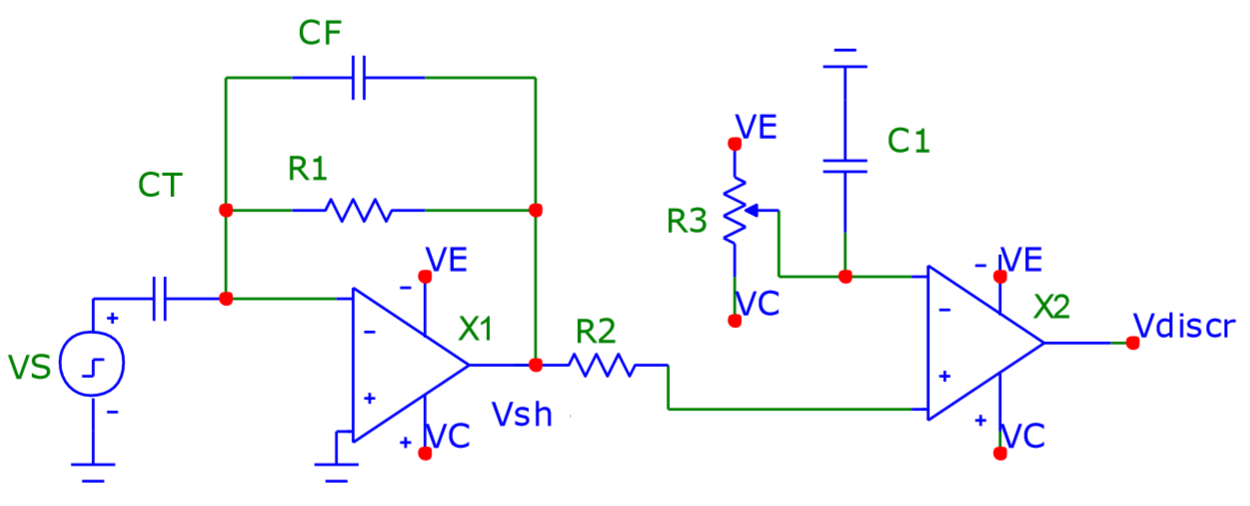
\includegraphics[scale=0.5]{amplificatoreCarica.png}
\caption{Amplificatore di carica realizzato con un OpAmp modello TL081.\label{circuito2}}
\end{figure}

\subsection*{1. Descrizione del circuito e prime misure}
Il circuito montato è costituito da tre parti distinte: un circuito di iniezione di carica ($V_S$+$C_T$), un circuito formatore che converte la carica in un segnale di forma fissata (X1) e un discriminatore che confronta il circuito con una soglia prefissata (X2).

La prima parte è costituita dal generatore di forme d'onda $V_S$ e dal condensatore $C_T$, dove viene fornita una carica pari a $Q_{IN}=V_S C_T$. Il formatore invece è rappresentato dal parallelo di $C_F$ e $R_1$, all'uscita di tale circuito si ha un segnale:\\
\begin{center}
$V_{SH}=\frac{Q_{IN}}{C_F} e^{-\frac{t}{\tau}} = V_S \frac{C_T}{C_F} e^{-t/R_1 C_F}$\\
\end{center}

Il resto del circuito rappresenta il discriminatore, analogo a quello descritto al punto A, ma con una tensione di soglia diversa da zero e determinata dal potenziometro. I componenti $R_2$ e $C_1$ hanno il compito di disaccoppiare il circuito formatore da quello discriminatore e di ridurre il rumore sulla tensione di soglia ad alte frequenze.\\
A frequenza fissata $f = 100\pm 1 \, Hz$ si è misurata la risposta del circuito ad un segnale di ampiezza picco-picco $V_S = 6.00 \pm 0.04 \, V$.\\
L'ampiezza massima attesa per il segnale $V_{SH}$, secondo la formula sopra citata, è $V_{SH.MAX.ATT} = V_S \frac{C_T}{C_F} =  5.9 \pm 0.3 \, V$, mentre il valore misurato sperimentalmente è $V_{SH.MAX} = 5.72 \pm 0.04 \, V$, come si vede in figura \ref{esponenziale}.\\

\begin{figure}[h]
\centering
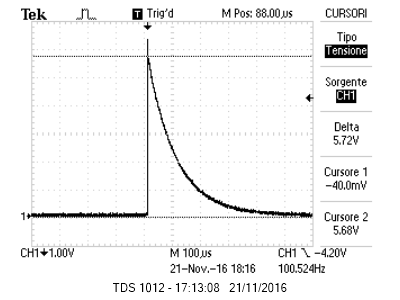
\includegraphics[scale=1.0]{immagini/esponenziale.png}
\caption{Misura del massimo valore dell'esponenziale $V_{SH.MAX.}$}
\label{esponenziale}
\end{figure}

Si sono misurati sull'oscilloscopio il tempo impiegato dal segnale $V_{sh}$ a scendere sotto i  $200 \, mV$ (fig. \ref{tempoEspo}) e il tempo per cui il segnale di uscita $V_{discr}$ è alto (\ref{tempoUscita}), i due valori sono $t_1 = 340 \pm 4 \, \mu s$ e  $t_2 = 336 \pm 4 \mu s$ rispettivamente e come si vede sono compatibili tra di loro.

\begin{figure}[h]
\centering
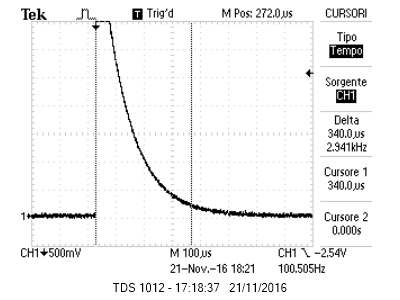
\includegraphics[scale=1.0]{immagini/periodoEsponenziale.png}
\caption{Tempo $t_1$ impiegato dall'ingresso del discriminatore a scendere sotto soglia.}
\label{tempoEspo}
\end{figure}

\begin{figure}[h]
\centering
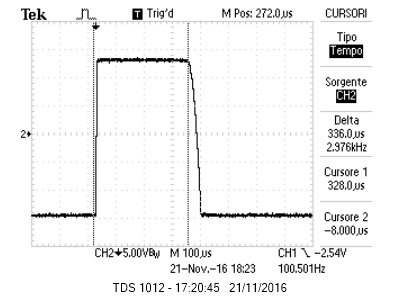
\includegraphics[scale=1.0]{immagini/tempoQuadra.png}
\caption{Tempo $t_2$ in cui l'uscita del discriminatore si mantiene positiva.}
\label{tempoUscita}
\end{figure}

\rem{Dire perchè il condensatore si carica a +6 e non a +3!!}


\subsection*{2. Dipendenza del segnale in uscita dall'ampiezza del segnale in ingresso}

Sempre mantenendo una frequenza fissa $f = 100 \pm 1 \, Hz$, si è misurata, al variare dell'ampiezza, la durata nel tempo del segnale in uscita dal discriminatore, i dati sono riportati nella tab. \ref{dati}, insiemi ai valori attesi, ricavati dalla $V_-=V_S \frac{C_T}{C_F} e^{- \Delta t/R_1 C_F}$, che invertendo si scrive: $\Delta t = -R_1 C_F log\left( \frac{V_- C_F}{V_S C_T}\right)$.

\begin{table}[!ht]
\centering
\begin{tabular}{|c|c|c|c|}
\hline 
• & $V_{IN} (V)$ & $\Delta t _ {atteso} (\mu s)$ & $\Delta t _ {misurato} (\mu s)$ \\ 
\hline
1 & $7.00 \pm 0.06$ & $355 \pm 11$ & $350 \pm 4$ \\
2 & $6.00 \pm 0.06$ & $340 \pm 10$ & $336 \pm 4$ \\  
3 & $5.00 \pm 0.04$ & $321 \pm 10$ & $317 \pm 4$ \\  
4 & $4.00 \pm 0.04$ & $300 \pm 10$ & $293 \pm 4$ \\ 
5 & $2.98 \pm 0.04$ & $270 \pm 8$ & $263 \pm 4$ \\ 
6 & $2.00 \pm 0.01$ & $230 \pm 8$ & $220 \pm 4$ \\ 
7 & $1.01 \pm 0.01$ & $160 \pm 5$ & $145 \pm 4$ \\   
\hline 
\end{tabular} 
\label{dati}
\end{table}


\rem{Aggiungere dati e fare un fit.}

I dati di tempo presi sono in accordo con quelli calcolati teoricamente.

Per una tensione in ingresso di $330 \, mV$ si vede che il segnale in uscita dall'amplificatore di carica perde la forma d'onda quadra e incomincia a diventare sinusoidale (fig. \ref{inizamorire}), per una tensione in ingresso che scende sotto il valore di soglia di $200 \, mV$ il trigger non si attiva, come si vede in figura \ref{morto}.

\begin{figure}[h]
\centering
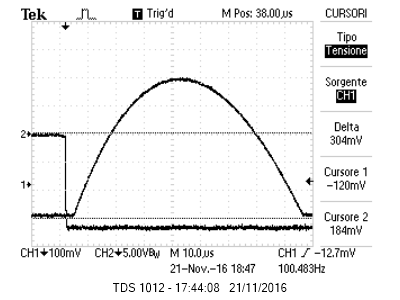
\includegraphics[scale=1.0]{immagini/iniziaamorire.png}
\caption{Tensione in ingresso al trigger del valore di $300 \, mV$.}
\label{inizamorire}
\end{figure}

\begin{figure}[h]
\centering
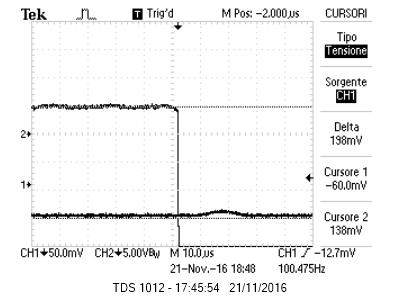
\includegraphics[scale=1.0]{immagini/morto.png}
\caption{Tensione in ingresso al trigger del valore di $300 \, mV$.}
\label{morto}
\end{figure}

\section*{C. Trigger di Schmitt}
\subsection{1. Montaggio, descrizione del circuito e valutazione tensioni di soglia}
Si è montato il circuito in fig. \ref{circuito3} con $R_1 = 9.92\pm0.08 \, k\Omega$ e $R_2 = 2.14 \pm 0.03 \, k\Omega$, alimentando l'operazionale con $V_{CC} = 14.96\pm0.08 \, V$ e $V_{EE} = 14.96 \pm 0.08 \, V$.\\

\begin{figure}[h]
\centering
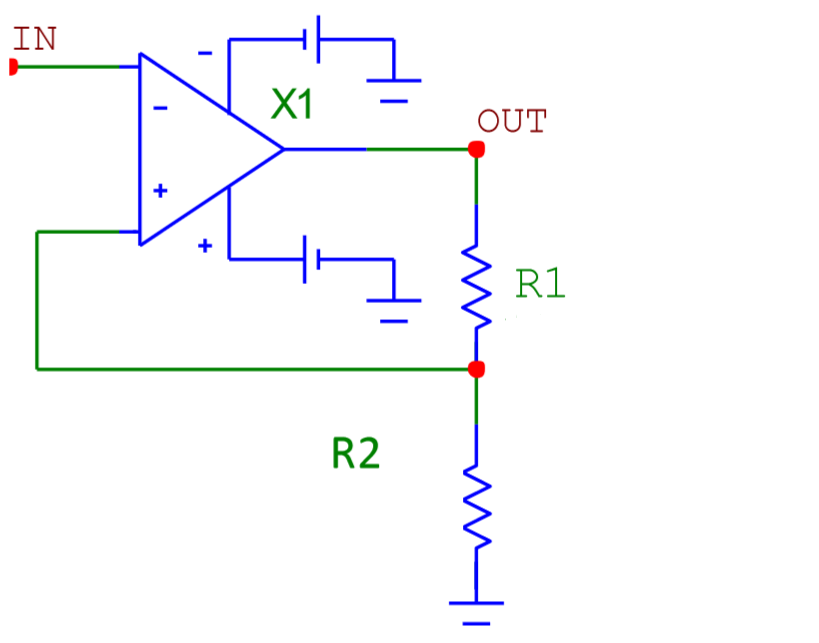
\includegraphics[scale=0.5]{triggerSchmitt.png}
\caption{Trigger di Schmitt realizzato con un OpAmp modello TL081.\label{circuito3}}
\end{figure}

In questo trigger grazie alla caduta di potenziale sulla resistenza $R_2$ del partitore costituito da $R_1$ e $R_2$, che viene immessa al $V_{+}$ dell'opAmp ogni volta che si ha un attraversamento della soglia ($V_{+}$) da parte del segnale immesso su $V_{-}$ la soglia stessa cambia (perchè cambia l'uscita $V_{OUT}$ e quindi la caduta di poteziale $V_{+}$). Pertanto dopo una commutazione perchè l'uscita cambi nuovamente è necessario che l'ingresso superi la seconda soglia, questo rende il discrimintore stabile rispetto al rumore del segnale in ingresso.

Al circuito è stata inviata in ingresso una tensione sinusoidale a frequenza di circa $f \sim 710 \pm 7 \, Hz$, e si sono misurate le tensioni in uscita nei due stati possibili: $V_{OH} = 14.5\pm 0.2 \, V$ e $V_{OL} = 14.0\pm0.2 \, V$ (inferiori alle tensioni di alimentazione), dalle quali si sono ricavati i valori attesi per le tensioni di soglia $V_{1,ATT,TH}= -V_{OH}/(1+R_1/R_2)= -2.57 \pm 0.05 \, V$ e $V_{2,ATT,TH}= V_{OL}/(1+R_1/R_2) = 2.48 \pm 0.05 V$. 

Dalle immagini fig. \ref{sogliameno} e fig. \ref{sogliapiu}, misurando a quale tensione dell'ingresso si ha la commutazione dell'uscita si sono trovati i due valori per le soglie: $V_{th, -} =-2.60 \pm 0.04 \, V $ e $V_{th, +} = +2.48 \pm 0.04 \, V$.

\begin{figure}[h]
\centering
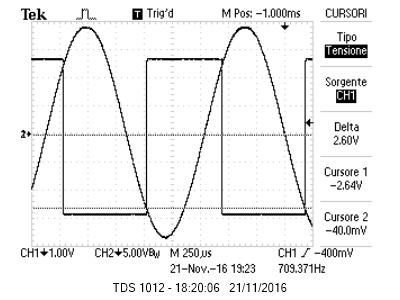
\includegraphics[scale=1.0]{immagini/FotoRicordoVth1.png}
\caption{Misura della soglia inferiore del trigger.}
\label{sogliameno}
\end{figure}

\begin{figure}[h]
\centering
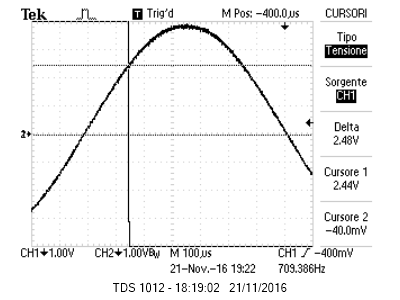
\includegraphics[scale=1.0]{immagini/FotoRicordoVth2.png}
\caption{Misura della soglia superiore del trigger.}
\label{sogliapiu}
\end{figure}

I valori delle tensioni di \emph{threshold} misurati sono in accordo con quelli stimati teoricamente entro gli errori.

\subsection*{2. Dipendenza dall'ampiezza e dalla frequenza e limiti del circuito}

Diminuendo l'ampiezza in ingresso questo non attraversa mai le soglia inferiore del trigger a $-2.60\,V$, come si vede nella fig. \ref{sottoSoglia}, quindi il segnale in uscita dal trigger rimane sempre basso (anche quando l'ampiezza in ingresso è diminuita tanto da non attraversare nemmeno la soglia a $+2.48\,V$).\\
Chiaramente aumentando l'ampiezza non si ha un comportamento simile per la soglia superiore perchè se il segnale attraversa la soglia a $-2.60\,V$ esso attraversa anche quella a $+2.48\,V$. L'uscita satura al valore superiore solamente se si aggiunge un \emph{offset} verso il basso e si diminuisce l'ampiezza, così che il segnale possa attraversare la soglia a $-2.60\,V$ senza attraversare quella a $+2.48\,V$.

\begin{figure}[h]
\centering
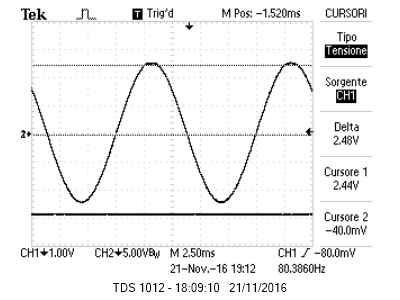
\includegraphics[scale=1.0]{immagini/sottoSogliaInferiore.png}
\caption{Segnale in ingresso che non attraversa la soglia inferiore del trigger a $-2.60V$.}
\label{sottoSoglia}
\end{figure}

Aumentando la frequenza  lo \emph{slew rate} è il fattore limitante dell'uscita del trigger, come si vede dalla risposta a forma di onda trapezoidale della fig. \ref{slew}, presa a $f = 323 \pm 3 \, kHz$. \\
Salendo in frequenza la pendenza del segnale satura, raggiunta questa condizione si è misurato lo \emph{slew rate} come rapporto incrementale: $dV = 8.00 \pm 0.08 \, V$ e $dt = 730 \pm 10 ns$, dai quali si ottiene \emph{slew rate} = $10.9 \pm 0.2 \, \frac{V}{\mu s}$, confrontabile con tutti i valori ottenuti nelle altre esperienze. Diminuendo la frequenza non si sono osservate deviazioni dal comportamento ideale degli opAmp. \\
Perchè il circuito lavori bene come trigger è necessario che sia $T >> \frac{V_{OH}+V_{OL}}{slew rate}$, cioè il periodo dell'onda da triggerare sia molto minore del tempo di commutazione.
\rem{Non ho mai considerato il 3\% sulle misure del'oscilloscopio ma va bene così}

\begin{figure}[h]
\centering
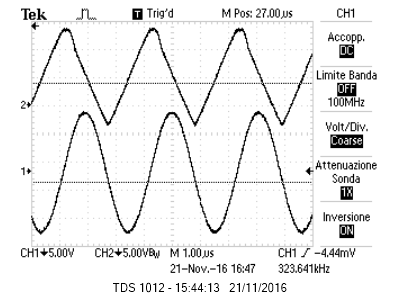
\includegraphics[scale=1.0]{immagini/slewRate.png}
\caption{Trigger di Schmitt ad alta frequenza e limitazione dovuta allo \emph{slew rate}}
\label{slew}
\end{figure}

\section*{D. Multivibratore astabile}
\subsection*{1. Analisi e montaggio del circuito}

Un circuito multivibratore astabile (come quello in fig. \ref{circuito4}) può essere realizzato partendo dal trigger di Schmitt inserendo all'uscita un ramo contenente due diodi Zener (e una resistenza $R_3$), insieme a un circuito RC (che determina l'instabilità e la frequenza di oscillazione).\\

\begin{figure}[h]
\centering
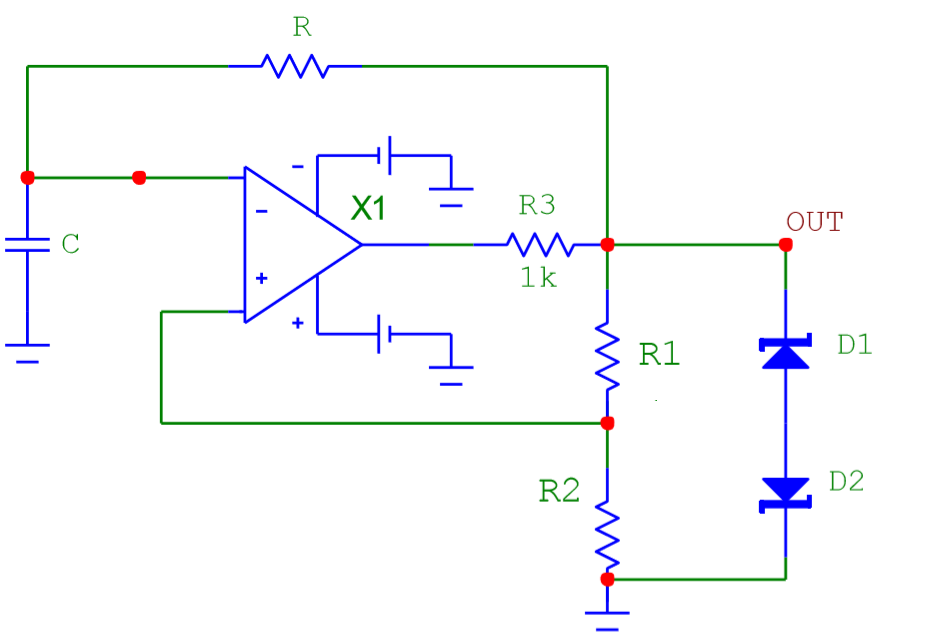
\includegraphics[scale=0.5]{multivibratoreAstabile.png}
\caption{Multivibratore astabile realizzato con un OpAmp modello TL081.\label{circuito4}}
\end{figure}

\subsection*{2. Breve spiegazione circuito oscillatore}

\begin{figure}[htb!]
\centering
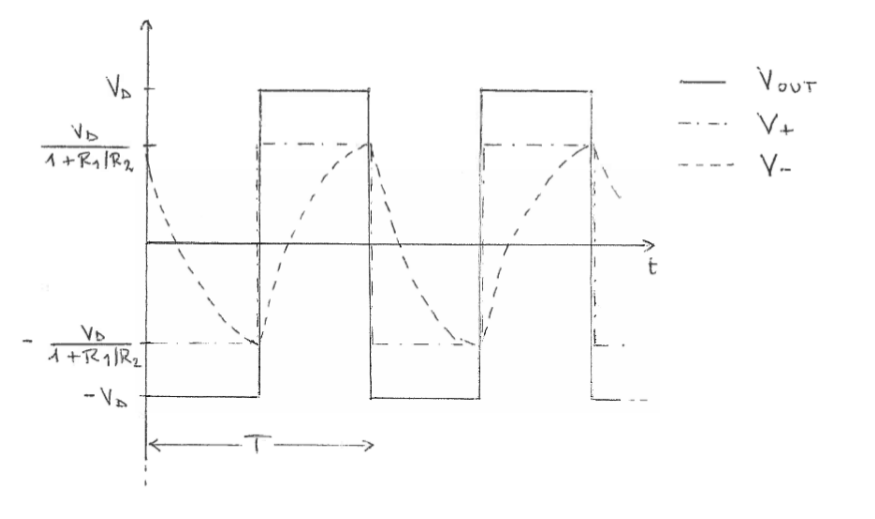
\includegraphics[scale=.5]{funzionamentoOscillatore.png}
\caption{Segnali del multivibratore.}
\label{funzionamento}
\end{figure}

Il condensatore inizialmente carico si scarica sulla resistenza $R$ per raggiungere $-V_D$, finchè non raggiunge la tensione di \emph{threshold} inferiore del trigger (data da $V_{+}$), allora la tensione in uscita commuta a $+V_{D}$ e anche il \emph{threshold} cambia (principio del trigger di \emph{Schmitt}), il condensatore si carica per raggiungere la tensione $V_D = V_{OUT}$, ma quando raggiunge la tensione di \emph{threshold} superiore l'uscita commuta nuovamente e il condensatore ricomincia a scaricarsi. Il tempo caratteristico dell'oscillazione è determinato da $\tau = RC$.\\

Si è determinato il periodo di oscillazione in funzione degli elementi resistivi: 
\begin{center}
$T=2\tau\, log\left( 1\,+\,2\frac{R_2}{R_1}\right) = 1.94 \pm 0.08 \, ms$ 
\end{center}
Dunque per ottenere un periodo dell'onda quadra di $\simeq 2 \, ms$ si deve scegliere $\tau = RC\simeq 0.9\,ms$.\\
A questo punto abbiamo potuto montare il circuito con $R = 3.87 \pm 0.04 \, k\Omega$, e un condensatore $C = 229 \pm 9 \, nF$, $R_1\,= 9.78\pm0.08 \, k\Omega $, $R_2 = 9.80\pm0.08\, k\Omega $ e $R_3 = 0.961\pm0.008 \, k\Omega $, con un' alimentazione per l'OpAmp di $V_{CC} = 14.96\pm0.08 \, V$ e $V_{EE} = 14.96 \pm 0.08 \, V$.


\subsection*{3. Verifica funzionamento del circuito}

I diodi Zener servono per limitare la tensione $V_{OUT}$, che satura tra i due valori estremi $\pm V_{D}$, dove $V_{D} = V_{Z} + V_{ \gamma}$. Per il diodo Zener $V_Z \sim 6.2 \, V$ \footnote{Il costuttore non fornisce incertezza.} e $V_{\gamma} \sim 0.7\, V$, dunque $V_D \sim 6.9 \, V$. \\
La tensione in uscita all'opAmp è vincolata alle tensioni di alimentazione ($\pm 15 \, V$), quindi tra l'uscita e il ramo dei diodi Zener vi è una caduta di potenziale pertantobisogna inserire una resistenza $R_3$ per evitare che i diodi si brucino a causa del passaggio di corrente elevato. \\ 

Sappiamo che le tensioni di \emph{threshold} superiore e inferiore per il trigger di \emph{Schmitt} sono: $V_{TH} = \pm \frac{V_{D}}{1+\frac{R1}{R2}} = \pm 3.45 \pm 0.05 \, V$, 
Ci aspettiamo per $V_{+}$ un'onda quadra la cui tensione picco-picco attesa è $V_{+, pp} = 6.9 \pm 0.1 \, V$, $V_{-}$ è costituito da cicli di carica e scarica del condensatore (quindi funzioni esponenziali) tra le tensioni di \emph{threshold}, quindi $V_{-, pp} = 6.9 \pm 0.1 \, V$. Essendo $V_{OUT}$ variabile tra $+V_{D}$ e $-V_{D}$, ci aspettiamo un'onda quadra con $V_{OUT, pp} \sim 13.8 \, V$.

Nelle fig. \ref{Vpiu}, \ref{Vout}, \ref{Vmeno} si vedono i segnali $V_{+}$, $V_{OUT}$ e $V_{-}$.\\

\begin{figure}[htb!]
\centering
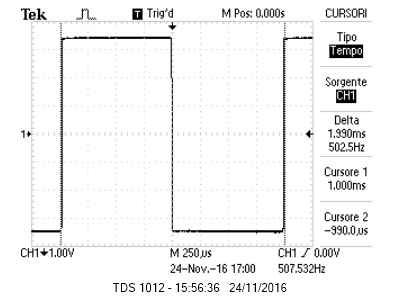
\includegraphics[scale=1.0]{immagini/multivibratoreVPIU.png}
\caption{Segnale $V_{+}$ dell'opAmp.}
\label{Vpiu}
\end{figure}

Il segnale $V_{+}$ (fig. \ref{Vpiu}) ha ampiezza picco-picco pari a $V_{+, pp} = 6.84 \pm 0.04\, V$, in buon accordo con il valore atteso. Il periodo misurato è $T = 1.99 \pm 0.01 \, ms$, anch'esso in accordo con il valore calcolato teoricamente.


\begin{figure}[htb!]
\centering
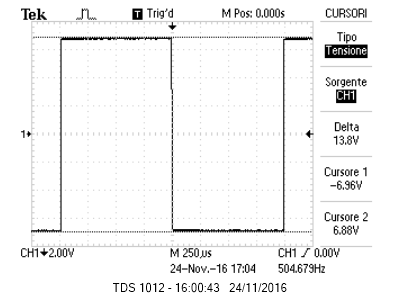
\includegraphics[scale=1.0]{immagini/multivibratoreVOUT.png}
\caption{Segnale $V_{out}$ dell'opAmp.}
\label{Vout}
\end{figure}

Si misura dalla fig. \ref{Vout}: $V_{OUT, pp} = 13.8 \pm 0.1\, V$, in ottimo accordo con quanto atteso.

\begin{figure}[htb!]
\centering
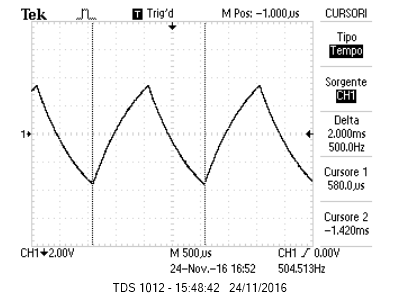
\includegraphics[scale=1.0]{immagini/multivibratoreVMENO.png}
\caption{Segnale $V_{-}$ dell'opAmp.}
\label{Vmeno}
\end{figure}

In fig. \ref{Vmeno} i tempi di carica e scarica del condensatore sono identici e pari a $t_{salita} = t_{discesa} = 1.00 \pm 0.02\, ms$, e il valore della tensione è: $V_{-, pp} = 6.96 \pm 0.04 \, V$, anche questi valori sono in accordo con quelli attesi.


\subsection*{4. Dipendenza dalla tensione di alimentazione}
Variando la tensione di alimentazione dell'opAmp \footnote{Restando nell'intervallo di tensioni di alimentazione indicati dal \emph{datasheet}, cioè non minori di $11\,V$ in valore assoluto.} non osserviamo significative variazioni del periodo dell'oscillatore perchè esso dipende solo dai valori delle resistenze e dei condensatori e non dalle alimentazioni. 


\subsection*{5. Limitazioni alla frequenza del segnale in ingresso}
Il funzionamento ad alta frequenza dell'oscillatore è limitato dallo \emph{slew rate}, in quanto l'opAmp esegue la commutazione tra i valori $\pm V_{D}$ in un tempo finito che deve essere molto minore del periodo di oscillazione del circuito.

\begin{figure}[htb!]
\centering
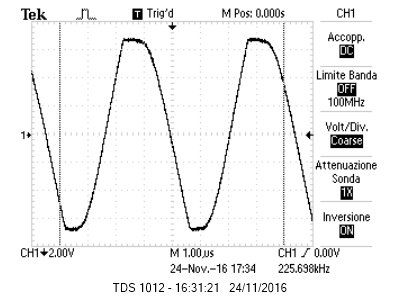
\includegraphics[scale=1.0]{immagini/multivibSlewRate.png}
\caption{Limitazioni dello \emph{slew rate} sul tempo di commutazione.}
\label{slewrate}
\end{figure}

Per valutare questo effetto abbiamo diminuito il valore di $\tau$ finchè non è diventato confrontabile con il valore del tempo di commutazione come si vede in fig. \ref{slewrate}. Quindi per $C = 0.099 \pm 0.004\, nF$ si è misurata la pendenza del segnale nell'intervallo di commutazione: $dV = 2.00 \pm 0.04 \, V$ e $dt = 192 \pm 4 \, ns$, da cui \emph{slew rate} = $10.3 \pm 0.3 \, \frac{V}{\mu s}$.\\
Possiamo concludere che l'oscillatore funziona bene per frequenze $f << \frac{1}{\Delta t} \sim \frac{1}{1 \, \mu s} = 1 \, MHz$, infatti il tempo di commutazione $\Delta t$ come si vede dalla fig. \ref{slewrate} è ci circa $\Delta t = 1 \, \mu s$.

\end{document}